\section{Donoremission nach Akzeptorbleichen}
In diesem Versuchsteil soll die FRET-Effizienz an CFP/YFP markierten Zellen bestimmt werden, indem 
die Donorfluoreszenz vor und nach dem Photobleaching des Akzeptormoleküls gemessen wird. \\
Während dem Bleichvorgang wird (idealerweise) nur der Akzeptor mit einem Laser der Wellenlänge 514 nm bei 
100\% Intensität bestrahlt und somit wird die Fluoreszenz des Akzeptors YFP verringert. \\
Während dem Versuch werden erst 10 Bilder vor dem Bleichen aufgenommen. Im nächsten Schritt
werden weitere 5 Bilder aufgenommen, diese stellen den Bleichvorgang dar. Zuletzt werden noch einmal 10 Bilder aufgenommen, 
um die Zelle nach dem Bleichvorgang auswerten zu können.\\
Um aus diesen Bildern die mittleren Intensitäten mithilfe des Messprogramm zu bekommen, werden sogenannte \textit{region of interest} (ROI) bestimmt. 
Die erste ROI 1 enthält immer den vollständig bestrahlten Bereich der Zelle während dem Bleichvorgangs. 
Die zweite ROI 2 wird um die Membran gezogen. 
Bei der dritten ROI 3 wird ein Ort in der Zelle gewählt, der sich durch besonders hohe Fluoreszenz auszeichnet. Bei einigen  
Messungen kam es hierbei allerdings zu einer unterschiedlichen Anzahl von ROI 3. Damit die 
verschiedenen Zellen besser vergleichbar sind,
wurden die ROI jeweils nach dem oben beschrieben Kriterien ausgewählt.\\
Um die ROI zu verdeutlichen, soll die folgende Graphik als Beispiel für die aufgenommenen Bilder
während dem Versuch dienen.\\
\begin{figure}[h]
    \centering
    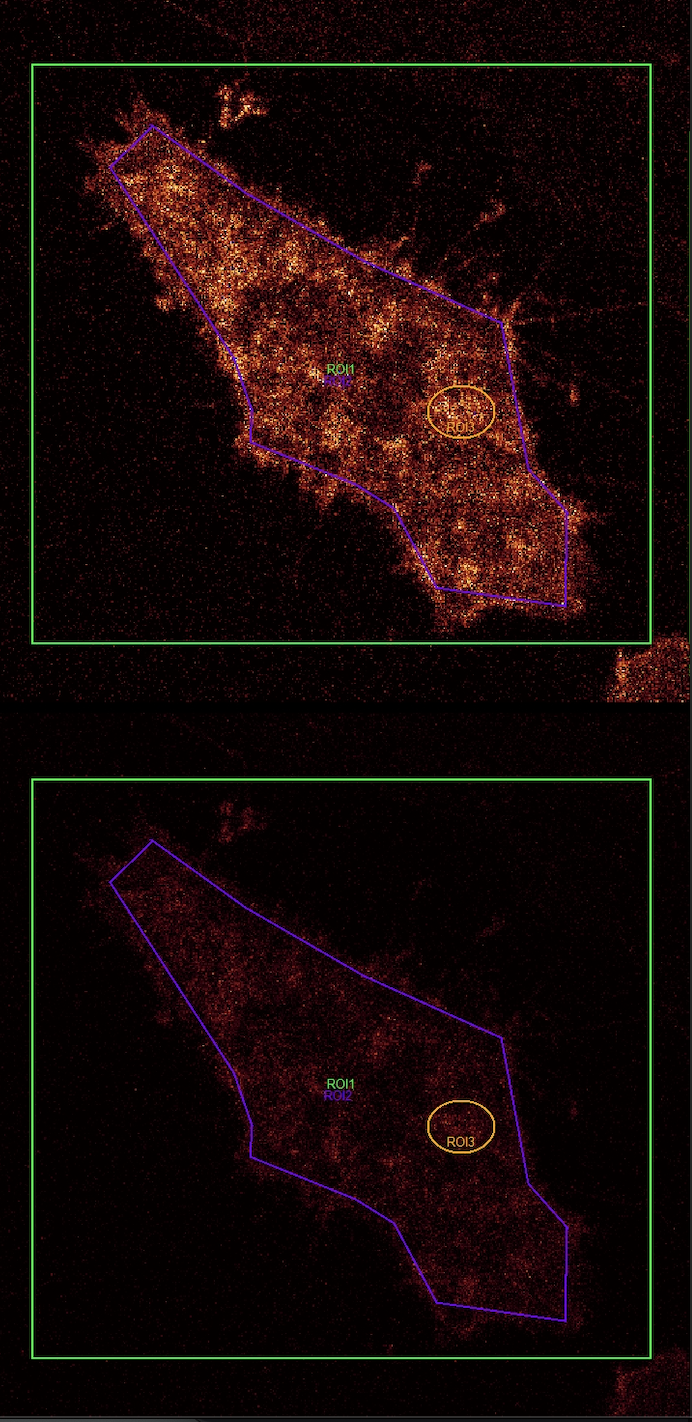
\includegraphics[scale=0.5]{Bilder/Auswertung_Anna/beispiel.PNG}
    \caption{Zelle 06 der YFP/CFP Probe vor und nach dem Bleichvorgang, unterteilt in verschiedenen ROI.}
    \label{fig:Beispeil}
   \end{figure}
\newpage
Das erste Bild steht hierbei für die Aufnahme vor dem Photobleaching und das zweite zeigt eine Aufnahme danach.
An diesen Bildern erkennt man die oben beschrieben ROI. Das grüne Rechteck steht für die ROI 1, die pinke Ummantelung für ROI 2
und der orangene Kreis für ROI 3, einen Bereich mit hoher Fluoreszenz innerhalb der Membran. \\\\
Zuerst wurden die Proben mit CFP und YFP markierten Zellen untersucht, anschließend
die nur CFP Proben und zuletzt die YFP Proben. Bei den ersten beiden Versuchsteilen wurde die 
Donorintensität betrachtet, im letzten Schritt allerdings die Akzeptorintensität. 
Nach der Mittelwertbildung wurden noch die Verhältnisse gebildet, um einen Vergleich 
ziehen zu können.
\subsection{CFP und YFP Proben}
Hier wurden zuerst über die Donorintensität $D_{CY,pre}$ vor der Akzeptorbleichung  
und die Donorintensität $D_{CY,post}$ nach dem Bleichvorgang für jede einzelne Zelle gemittelt. Anschließend 
wird die FRET-Effizienz E nach der im Skript angegeben Formel berechnet:
\begin{equation}
    E = 1 - \frac{D_{CY,pre}}{D_{CY,post}}
\end{equation}
Aus der folgenden Tabelle sind die entsprechenden Werte zu entnehmen:\\
\begin{table}[h]
    \centering
      \begin{tabular}{c|c|c|c}
      \textbf{Zelle} & \textbf{ROI 1} & \textbf{ROI 2} & \textbf{ROI 3} \\
      \hline
      \textbf{1} & 0,02  & 0,03  & 0,04 \\
      \textbf{2} & 0,02  & 0,04  & 0,07 \\
      \textbf{3} & 0,07  & 0,01  & 0,11 \\
      \textbf{4} & 0,04  & 0,07  & 0,13 \\
      \textbf{5} & 0,01  & 0,02  & -0,01 \\
      \textbf{6} & 0,10  & 0,10  & 0,06 \\
      \textbf{7} & -0,02 & -0,01 & 0,07 \\
      \textbf{8} & 0,01  & 0,03  & 0,07 \\
      \end{tabular}
      \caption{FRET-Effizienz, berechnet aus der Donorintensitäten (von CFP/YFP Proben) vor und nach dem Bleichvorgang für 8 Zellen.}
    \label{tab:FRET-Effizienz}
  \end{table}\\
Hierbei muss gesagt werden, dass die aufgeführten Werte nicht die kompletten Werte der Messung sind. 
Die erste Messung wurde in dieser Tabelle nicht mit aufgeführt, da hierbei nur zwei ROI gemessen wurden und 
somit der Vergleich der dritten ROI nicht gegeben war. Die dritte Messung wurde ebenfalls ausgeschlossen, 
da auch hier nur zwei ROI gemessen wurden. 
Die letzten Messungen wurden hier ebenfalls ausgelassen, da bei diesen Messungen nur die 
halbe Zelle gebleicht wurde. \\
Wenn man nun die verbliebenen Messungen betrachtet, fällt wie erwartet auf, dass 
ROI 1 die geringste Effizienz aufweist. Dies hat den Grund, dass dieses Gebiet nicht nur
die Zelle beinhaltet, sondern auch 'toten Raum', in diesem Raum befinden sich keine 
fluoreszierende Punkte. Ein 'Ausreißer' ist hier die Zelle 3, dies hat wahrscheinlich den Grund, 
dass bei unserer Aufnahme das Gebiet aus zwei Zellen besteht und nicht nur aus einer. \\
Allgemein fällt noch auf, dass die Werte sehr klein sind, dies kann man darauf zurückführen, dass die
Akzeptorbleichung nicht in der gewünschten Stärke (nach Anleitung sollten es mindestens 50\% sein) bei unserem Versuch möglich war. \\
Bei den negativen Ergebnissen kann man davon ausgehen, dass der Bleichvorgang, keine Wirkung auf 
die Zelle hatte.
\newpage
Eine deutlich höhere Effizienz hatte dabei allerdings der Bereich der Zellmembran ROI 2, da in diesem Bereich
auch eine deutlich höhere Ansammlung an CFP und YFP Proben vorliegt, diese fluoreszieren können. Somit scheint 
die höhere Effizienz, im Gegensatz zur ROI 1, plausibel.\\
Laut Theorie sollte der größte Wert der Effizienz in der ROI 3 zu finden sein, da diese auch dementsprechend gewählt wurde. 
Allerdings ist dies nicht immer der Fall, dies lässt sich auf die Tatsache zurückführen, 
dass die ROI 'per Auge' von uns während dem Versuch ausgewählt wurde und somit nicht garantiert werden kann, dass
es sich bei ROI 3 wirklich um das Gebiet mit der stärksten Bleichung handelt.\\\\
In dem folgenden Diagramm \ref{fig:plotA2} wird die Fluoreszenzintensität des Donors und des S.E. Channels 
gegen die Zeit aufgetragen. Dies wird beispielhaft an einer Zelle (Zelle 03) dargestellt und nur für die ROI 1.
Die grüne Linie beschreibt hierbei die Donorintensität. Diese Linie verläuft am Anfang
beinahe horizontal, dies ist die Zeit vor dem Bleichen. Während dem Photobleaching 
hat die CFP Probe keine Intensität, da diese bei dem Bleaching (idealerweise) auch nicht bestrahlt
wird. Es soll lediglich das Akzeptormoleküls gebleicht werden.
Nach der 'Lücke' ist die Linie wieder eine Gerade (parallel zur x-Achse), diese stellt den Zeitraum
nach dem Bleaching dar. \\
Die blaue Linie in der Grafik zeigt die Sensitized Emission. Wie man erkennen kann, 
verläuft diese ebenfalls parallel zur x-Achse vor dem Bleaching, allerdings fällt auf, 
dass die Intensität der S.E. Probe deutlich höher liegt als die zu vergleichende
Probe. Während dem Photobleaching steigt die blaue Linie sprunghaft an, 
dies ist plausibel, wenn man bedenkt, dass der Akzeptor mit voller 
Laser Intensität bestrahlt wird. Zuletzt sinkt die 
Linien wieder und setzt sich wieder als Gerade fort, da sich die Intensität 
nach dem Photobleaching nicht mehr großartig ändert.\\
Beide Intensitäten sind allerdings vor dem Bleaching höher als nachdem, dies entspricht den Erwartungen.\\
\begin{figure}[h]
\centering
  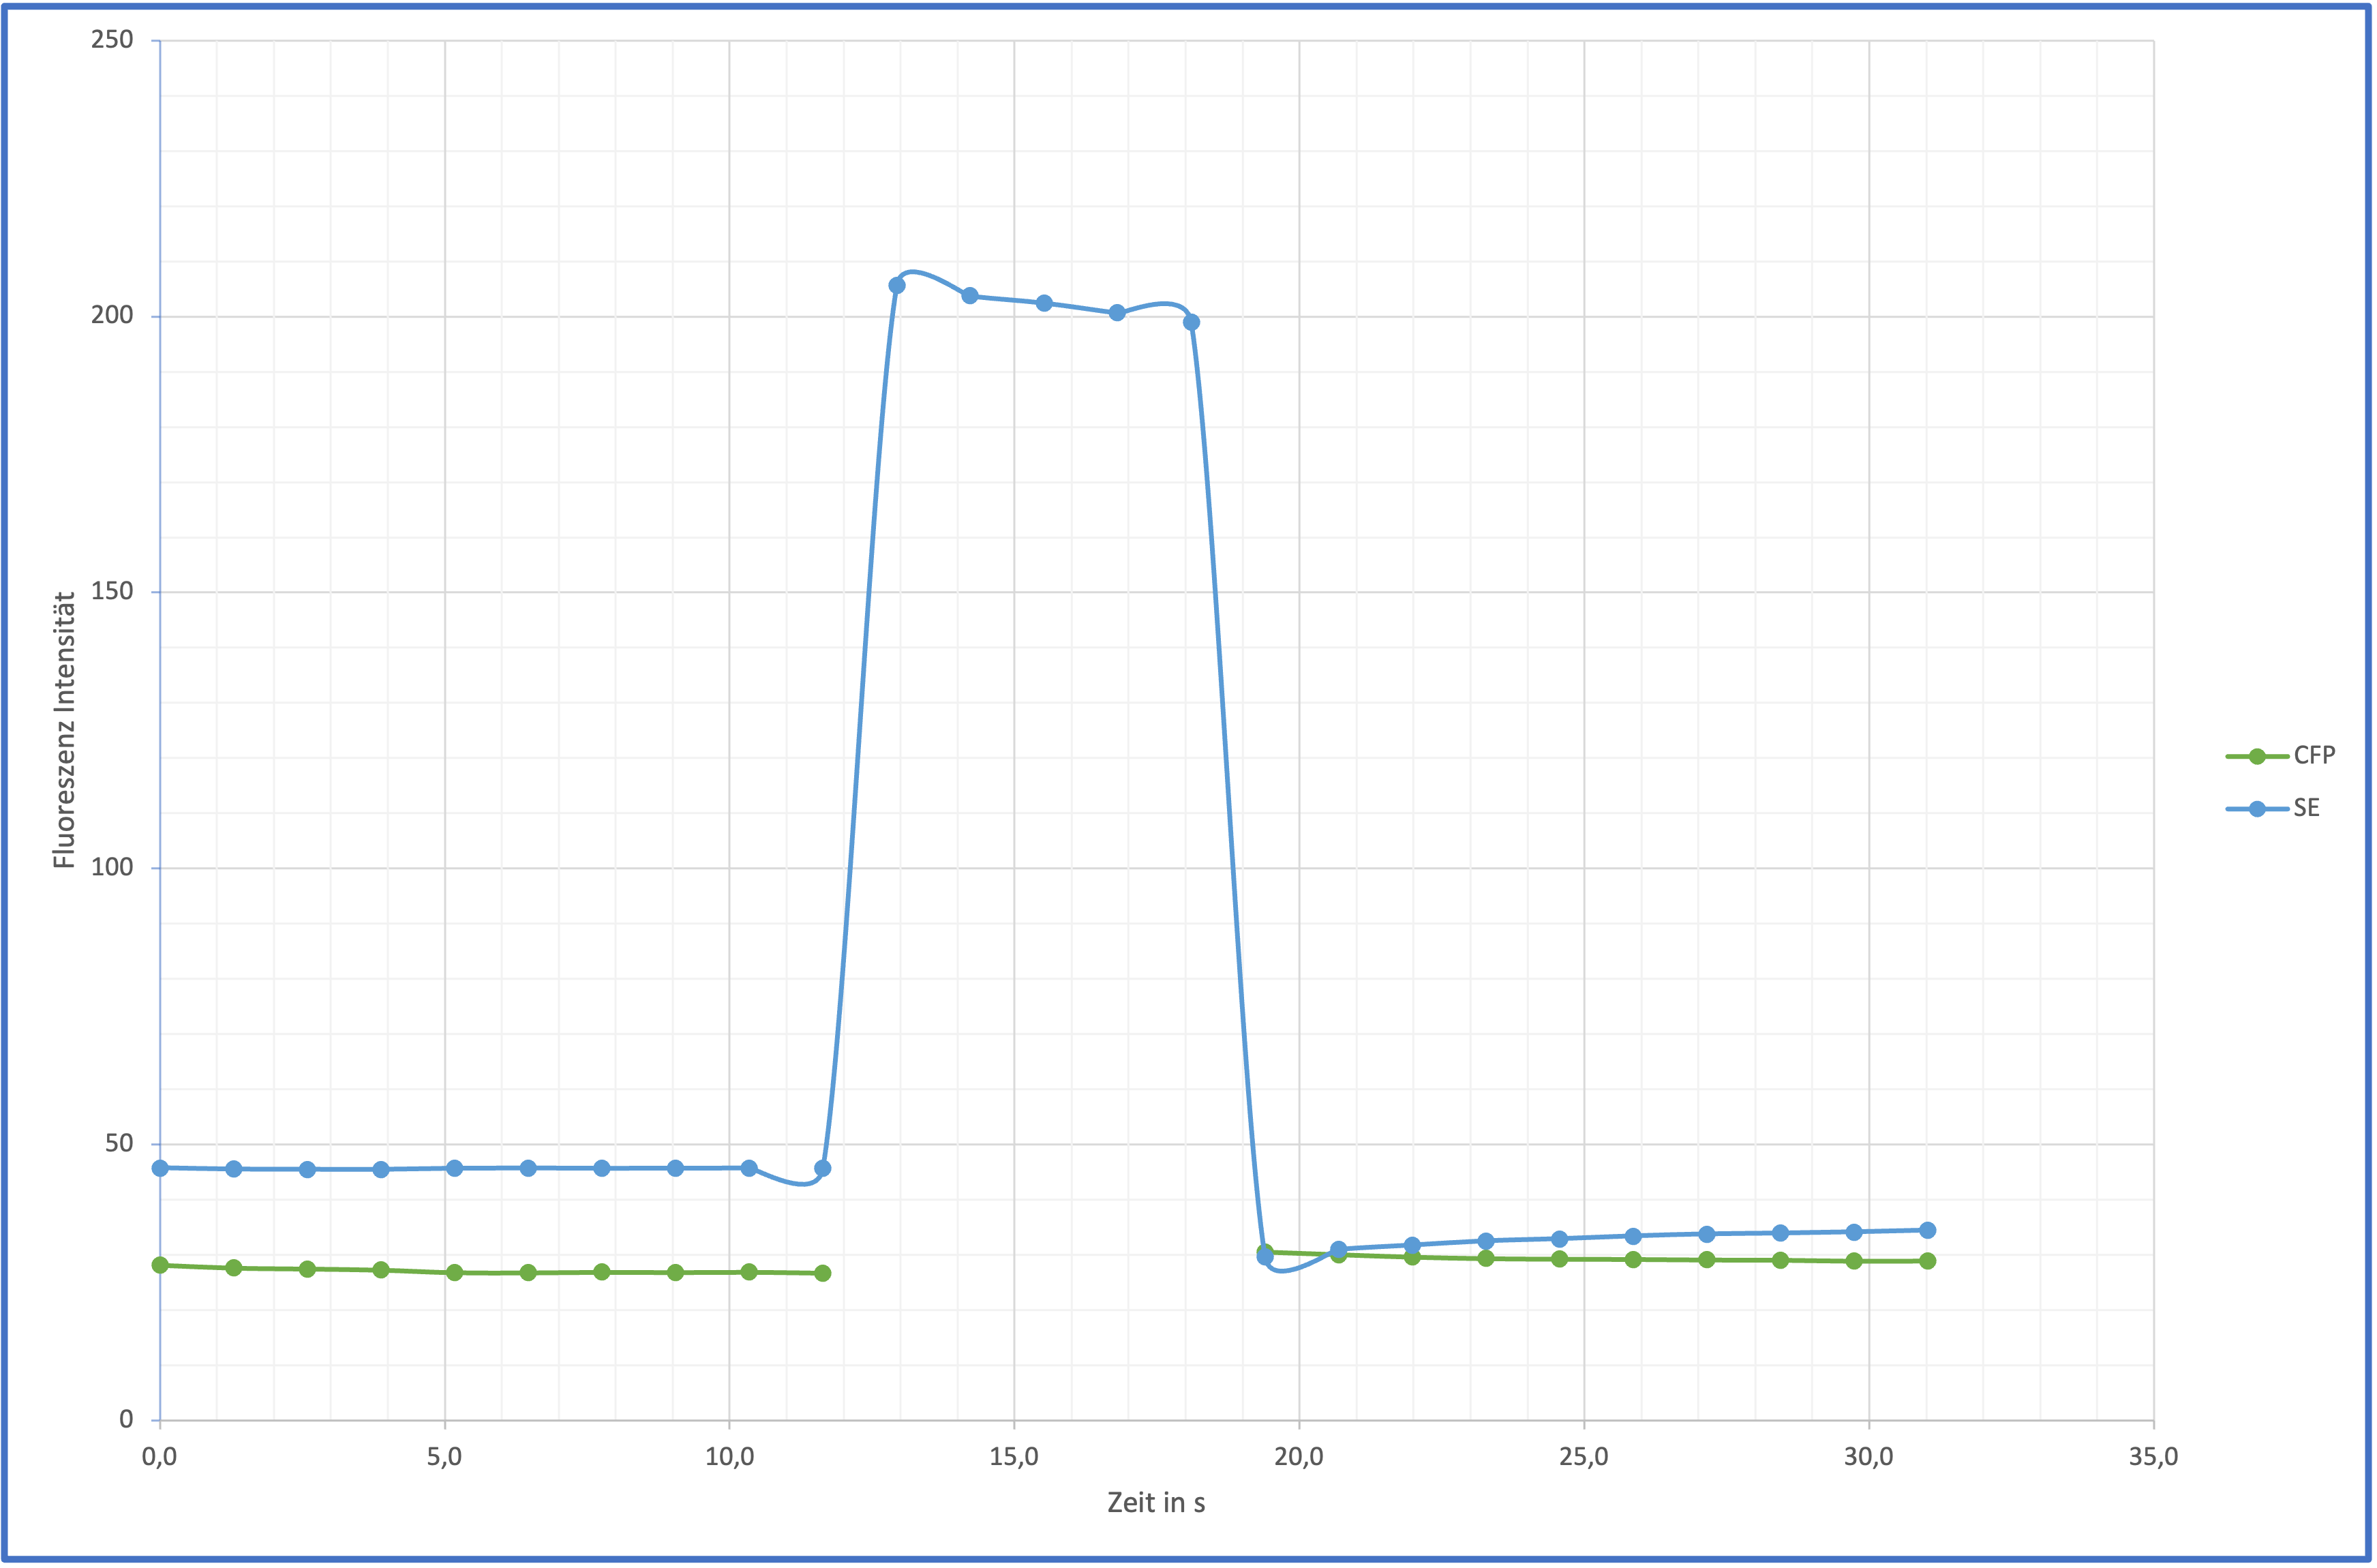
\includegraphics[scale=0.3]{Bilder/Auswertung_Anna/plot.PNG}
  \caption{Grafik über die Fluoreszenz Intensität vor, während und nach dem Photobleaching über einen Zeitraum. Blau: Sensitized Emission; Grün: Donorintensität}
  \label{fig:plotA2}
\end{figure}\\
\subsection{CFP-Proben}
Desweitern wurde die Akzeptorbleichung nur bei CFP-Proben aufgenommen, um einen Kontrollpunkt zu bekommen. 
Laut Theorie sollte es hier keinen Unterschied zwischen der Intensität vor und nach dem Bleichvorgang 
geben. Um dies zu untersuchen wird das folgende Verhältnis gebildet:
\begin{equation}
    V_1 = \frac{D_{CY,pre}}{D_{CY,post}}
\end{equation}
\newpage
Die Werte sind in der folgenden Tabelle aufgeführt:
\begin{table}[h]
    \centering
      \begin{tabular}{c|c|c|c}
      \textbf{Zelle} & \textbf{ROI 1} & \textbf{ROI 2} & \textbf{ROI 3} \\
      \hline
      \textbf{1} & 1,02  & 0,99  & 1,00 \\
      \textbf{2} & 1,03  & 1,02  & 1,09 \\
      \textbf{3} & 1,02  & 1,01  & 1,01 \\
      \textbf{4} & 1,01  & 1,01  & 1,05 \\
      \textbf{5} & 1,02  & 1,02  & 0,97 \\
      \textbf{6} & 1,00  & 1,01  & 1,02 \\
      \textbf{8} & 1,00  & 1,03  & 0,98 \\
      \textbf{9} & 1,03  & 0,89  & 1,04 \\
      \textbf{10} & 1,03  & 0,03  & 1,04 \\
      \textbf{11} & 1,00  & 1,03  & 1,01 \\
      \end{tabular}
      \caption{Verhältnis der Donorintensitäten einer reiner CFP Probe vor und nach der Bleichung für 3 ROI für je 11 Zellen.}
    \label{tab:Verhältnis CFP}
  \end{table}\\
  Wie man erkennt, stimmt die Theorie ziemlich gut mit dem Experiment überein, da die Werte nahe um 1 
  liegen. Das bedeutet, dass während dem Photobleaching zum größtenteils nur der Akzeptor gebleicht wurde.
\subsection{YFP-Proben}
Zuletzt wurde das Akzeptorbleichen auch auf reine YFP Proben angewendet. 
Hierbei wurde allerdings das Verhältnis der Akzeptorintensitäten vor und nach dem Bleaching betrachtet
und ins Verhältnis versetzt. 
\begin{equation}
    V_2 = \frac{A_{YFP,post}}{A_{YFP,pre}}
\end{equation}
Die Werte finden sich in der folgenden Tabelle:
\begin{table}[h]
    \centering
      \begin{tabular}{c|c|c}
      \textbf{Zelle} & \textbf{ROI 1} & \textbf{ROI 2} \\
      \hline
      \textbf{1} & 0,39  & 0,49 \\
      \textbf{2} & 0,38  & 0,46 \\
      \textbf{3} & 0,44  & 0,47 \\
      \textbf{4} & 0,71  & 0,67 \\
      \textbf{5} & 0,35  & 0,33 \\
      \textbf{6} & 0,29  & 0,38 \\
      \end{tabular}
      \caption{Verhältnis der Akzeptorintensitäten vor und nach dem Bleichvorgang einer reinen YFP Probe für 6 Zellen.}
    \label{tab:Verhältnis der Akzeptorintensitäten}%
  \end{table}%
  
Theoretisch sollte die Intensität nach dem Photobleaching deutlich geringer ausfallen, also davor. 
 Wie man erkennen kann, ist dies auch der 
Fall, allerdings fällt die Stärke des Photobleaching deutlich geringer aus als gefordert.\\\\
Zuletzt soll dieses Verfahren noch mit der vorangegangenen Methode verglichen werden. Die FRET-Effizienz Werte
der Sensitized Emission liegen deutlich höher (vgl. Tabelle \ref{tab:SE Effizienz}), als die Werte der FRET Effizienz der Akzeptorbleichung. \\
Ein generelles Problem, welches zu hohen Messunsicherheiten führt, ist das die ROI willkürlich während dem 
Versuch bestimmt werden. Ein Problem dieser Messmethode (Akzeptorbleaching) ist, dass nur ein Teil des YFP 
Moleküls gebleicht wird, wie die Tabelle \ref{tab:Verhältnis der Akzeptorintensitäten} zeigt. Dies 
führt zu dieser großen Abweichung der FRET Effizienz zwischen den verschiedenen Messmethoden.
